\documentclass{bioinfo}
\copyrightyear{2015}
\pubyear{2015}

\usepackage{amsmath}
\usepackage{natbib}
\usepackage{hyperref}

\usepackage{pdfpages}

\bibliographystyle{apalike}

\begin{document}
\firstpage{1}

\title[Metagenome-enabled error correction]{corsage: Metagenome-enabled error correction of single cell sequencing reads}

\author[Bremges \textit{et~al.}]{Andreas Bremges\,$^{1}$\footnote{to whom correspondence should be addressed}, Esther Singer\,$^{2}$, Tanja Woyke\,$^{2}$ and Alexander Sczyrba\,$^{1}$}

\address{$^{1}$Center for Biotechnology \& Faculty of Technology, Bielefeld University, 33615 Bielefeld, Germany\\
$^{2}$U.S. Department of Energy Joint Genome Institute, Walnut Creek, CA 94598, USA}

\history{Received on XXXXX; revised on XXXXX; accepted on XXXXX}
\editor{Associate Editor: XXXXXXX}
\maketitle

\begin{abstract}
\section{Summary:} We present a new tool, corsage, to correct sequencing errors in Illumina data produced from single amplified genomes (SAGs).
It uses sequence information derived from accompanying metagenome sequencing to accurately correct errors even in ultra-low coverage regions of the single cells.
In evaluations on real data, we show that corsage outperforms BayesHammer, the current (and widely used) state-of-the-art. %TODO
corsage particularly does well in correcting chimeric reads, which helps to improve both accuracy and contiguity of \emph{de novo} assemblies.

\section{Availability and implementation:} corsage is implemented in C and is freely available under the open source MIT license from \href{https://github.com/metagenomics/corsage}{https://github.com/metagenomics/corsage} %TODO

\section{Contact:} \href{mailto:abremges@cebitec.uni-bielefeld.de}{abremges@cebitec.uni-bielefeld.de}

%\section{Supplementary information:} Test data and in-depth evaluations are available from \href{https://github.com/metagenomics/2015-corsage}{https://github.com/metagenomics/2015-corsage} \textbf{XXX}
\end{abstract}

\vspace{-1em}

\section{Introduction}

The vast majority of microbial species observed in nature cannot be grown in pure culture \citep{rappe}, turning metagenomics and -- more recently -- single cell genomics into indispensable methods to study the microbial dark matter \citep{mdm}.
Frequently, single amplified genomes (SAGs) and accompanying shotgun metagenomes are generated from the same environmental sample \citep{mason, op9}, and were methodologically combined to validate metagenome bins with single cells \citep{cowrumen} or to improve the SAG's assembly contiguity \citep{sr1}.
But so far, noone explored the idea to combine both approaches to correct sequencing errors in single cell sequencing reads.

\textit{SAG reads pose additional challenges to error correction: uneven sequencing depth~\citep{chitsaz}, ultra-low coverage regions with basically no correction possible (Table~\textbf{S1}).} %TODO
\textit{Many chimeric reads \citep{lasken}, we expect one chimeric event every 10 kb \citep{rodrigue}, they pose a big challenge during assembly \citep{spades2}.} %TODO
While there are plenty of error correction tools for a variety of use cases available \citep{david}, only one tool was specifically designed to correct SAG data: hammer \citep{hammer}, developed further to BayesHammer \citep{bayeshammer}.

\textit{Conclude that one might want to use both data sources for the job. If an accompanying metagenome is available, you might as well take advantage of it!}

\vspace{-1em}

\begin{methods}
\section{Methods}

We correct potential sequencing errors using an algorithm similar to solving the \emph{spectral alignment problem}~\citep{euler}.
Given a set of trusted $k$-mers, we attempt to find a sequence with minimal corrections such that each $k$-mer on the corrected sequence is trusted.
We consider a $k$-mer trusted if it occurs at least $2\times$ in the accompanying metagenome. %TODO user-adjustable parameter, refer to supplement - erroneous $k$-mers tend to occur only once in the metagenome

In principle, corsage is similar to the error correction in fermi \citep{fermi}.
It differs in that it removes fermi's assumption of even sequencing coverage to account for the extreme coverage bias in single cell data.
Instead, it exploits metagenomic sequence information to correct errors even in ultra-low coverage regions of the single cell.
The metagenome generates coverage at sites with too low a coverage for SAG-only error correction.

corsage corrects errors in three phases:
\begin{enumerate}
\item corsage collects all 31-mers occurring in the SAG reads. It uses this information to initialize a hash table with the 31-mers being valid keys.
\item corsage scans the accompanying metagenomic reads. For each stored 31-mer, it counts the occurence of the next (i.e. the 32-nd) base in the metagenome and stores this information in the hash table. This step is largely I/O bound and dominates corsage's runtime (Table~\textbf{S2}). %TODO
\item corsage processes each SAG read by using the 31-mer hash table to check if the 32-nd base has sufficient support in the metagenome.
Roughly speaking, corsage tries to correct an unsupported base if by looking up its 31-mer prefix we know the base is different from an overwhelmingly frequent 32-nd base in the metagenome.
\end{enumerate}

\end{methods}

\section{Results and Discussions}

As a realistic benchmark, we used eight \textit{Escherichia coli} K12-MG1655 SAGs from~\citealp{scott2}, for which the complete genome sequence is available.
We generated an accompanying \emph{in vitro} mock metagenome consisting of 26 microbial species and sequenced it on Illumina's HiSeq (Table~\textbf{S2}). %TODO
Based on measured molarity (mapped metagenome reads), we estimate an abundance of $0.3\%$ ($0.24\%$) for \textit{E.~coli}, corresponding to a mean genome coverage of $20.7\times$. %TODO

\begin{table}[t]
\processtable{Performance of error correction}
{\footnotesize
%\begin{tabular}{p{1.1cm}p{1.5cm}p{1.4cm}p{1.5cm}p{1.4cm}} %.0
\begin{tabular}{lrrrr}
\toprule
Program  & \% perfect            & \% chimeric               & \% better             & \% worse \\
\midrule
%raw     & 22.5184 $\pm$ 1.06776 & 0.731692 $\pm$ 0.154783   & --                    & -- \\
raw      & 22.52 $\pm$ 1.07      & 0.73 $\pm$ 0.15           & --                    & -- \\
%hammer  & 80.3488 $\pm$ 8.76926 & 0.77009 $\pm$ 0.173177    & 71.6641 $\pm$ 2.12213 & 0.334178 $\pm$ 0.0552847 \\
hammer   & 80.35 $\pm$ 8.77      & 0.77 $\pm$ 0.17           & 71.66 $\pm$ 2.12      & 0.33 $\pm$ 0.06 \\
%corsage & 95.518 $\pm$ 0.427942 & 0.0594387 $\pm$ 0.0243216 & 75.4515 $\pm$ 1.11489 & 0.264937 $\pm$ 0.032874 \\
corsage  & \textbf{95.52 $\pm$ 0.43}      & \textbf{0.06 $\pm$ 0.02}           & \textbf{75.45 $\pm$ 1.11}      & \textbf{0.26 $\pm$ 0.03} \\
\botrule
\end{tabular}}{Refer to Table \textbf{S3}. %TODO
Give all versions and the non-default command-line arguments: corsage option `\mbox{-c 2}', BayesHammer-v3.6.0 quality trimming disabled via config file.
State that we use BWA-MEM \citep{bwamem} and samtools \citep{samtools}.
Given is the mean and std.dev for all 8 \textit{E. coli} SAGs, best in bold.
}
\end{table}

\begin{table*}[b]
\processtable{Effect on {\it de novo} assembly}
{\footnotesize
\begin{tabular}{llrrrrrrrrrr}
\toprule
Assembler & Corrector & NG50  & \# contigs & Largest contig & Total length  & MA    & MM    & IND  & GF (\%) & \# genes & NGA50 \\
\midrule
IDBA-UD   & raw       & 49982 & 394        & 186696         & 4410124       & 15.00 &  7.38 & 0.55 & 93.474  & 3846 & 49714 \\
          & hammer    & 48672 & 400        & 168302         & 4411299       & 14.88 &  7.69 & 0.62 & 93.425  & 3837 & 48653 \\
          & corsage   & \textbf{64127} & \textbf{327}        & \textbf{191229}         & \textbf{4422372}       &  \textbf{6.88} &  \textbf{5.72} & \textbf{0.40} & \textbf{93.877}  & \textbf{3919} & \textbf{64074} \\
\midrule
SPAdes    & raw       & 77752 & 473        & 212552         & \textbf{4531527}       & 18.88 & 21.88 & 1.82 & 94.247 & 3889 & 76859 \\
          & hammer    & 86615 & 369        & 222585         & 4472703       & 14.50 & 19.16 & 1.89 & 94.041  & 3902 & 85054 \\
          & corsage   & \textbf{87774} & \textbf{347}        & \textbf{228604}         & 4484817       &  \textbf{8.88} & \textbf{16.13} & \textbf{1.51} & \textbf{94.268}  & \textbf{3934} & \textbf{86690} \\
\botrule
\end{tabular}}{Refer to Table \textbf{S4} and \textbf{S5}. %TODO
%Here, give some definitions of the metrics.
Assembled with IDBA-UD-1.1.1~(\citealp{idba_ud}; default options) and SPAdes-3.6.0~(\citealp{spades1}; options `\mbox{-{}-sc} \mbox{-{}-only-assembler} \mbox{-{}-careful} \mbox{-k 21,33,55,77}').
Statistics computed with QUAST-3.0~(\citealp{quast}; default options).
Given is the mean for all 8 \textit{E. coli} SAGs, best in bold.
}
\end{table*}

We evaluated corsage along with BayesHammer~(\citealp{bayeshammer}), the current state-of-the-art. % to correct single cell sequencing reads (Table~1).
corsage corrects more errors than BayesHammer, producing a higher fraction of better and perfect reads after correction, while maintaining a high accuracy.
Notably, corsage also suppresses chimeric reads, potentially due to the metagenome not being MDA-amplified. BayesHammer surprisingly introduces additional chimeric reads.

corsage also works well with single cell assemblers (Table~2).
\textit{Discuss results obtained with SPAdes-3.6.0 \citep{spades1} and IDBA-UD-1.1.1 \citep{idba_ud}. Less misassembly events, probably because corsage corrects chimeric reads, too. Also slightly increased contiguity while maintaining or surpassing the original accuracy.}

\textit{Discuss outliers (6 \& 7), better MDA = less coverage bias = better assembly. Here, hybrid error correction shows the least effect.}
\textit{Point to the Table~\textbf{S1}.}
\textit{SAGs with highest MDA bias (3 \& 4) are harder to correct (more ultra-low coverage regions), and also perform poorest in assembly (Tables~\textbf{S4} and \textbf{S5}). These benefit the most from metagenome-enabled error correction.}
\textit{Incorporating a second source of information (metagenome) has the potential to expand the current state-of-the-art, and produces excellent results.}

\textit{Discuss, that metagenome-enabled error correction of SAG data might result in miscorrections of rare variants (low-abundant strain captured, reads might get corrected towards the most abundant strain).}
\textit{Argue that these do not matter much, and could be polished in a postprocessing step (e.g. pilon, sequel).}

\section*{Acknowledgement}
%Esther Singer, if she doesn't qualify as co-author (Tanja decides). She generated the mock metagenome. %TODO
\paragraph{Funding\textcolon}
AB is supported by a fellowship from the CLIB Graduate Cluster Industrial Biotechnology and is partially funded by the International DFG Research Training Group GRK 1906/1.
The work conducted by the U.S. Department of Energy Joint Genome Institute, a DOE Office of Science User Facility, is supported under Contract No. DE-AC02-05CH11231.

%%%%%%%%%%
\bibliography{corsage_refs}

\newpage
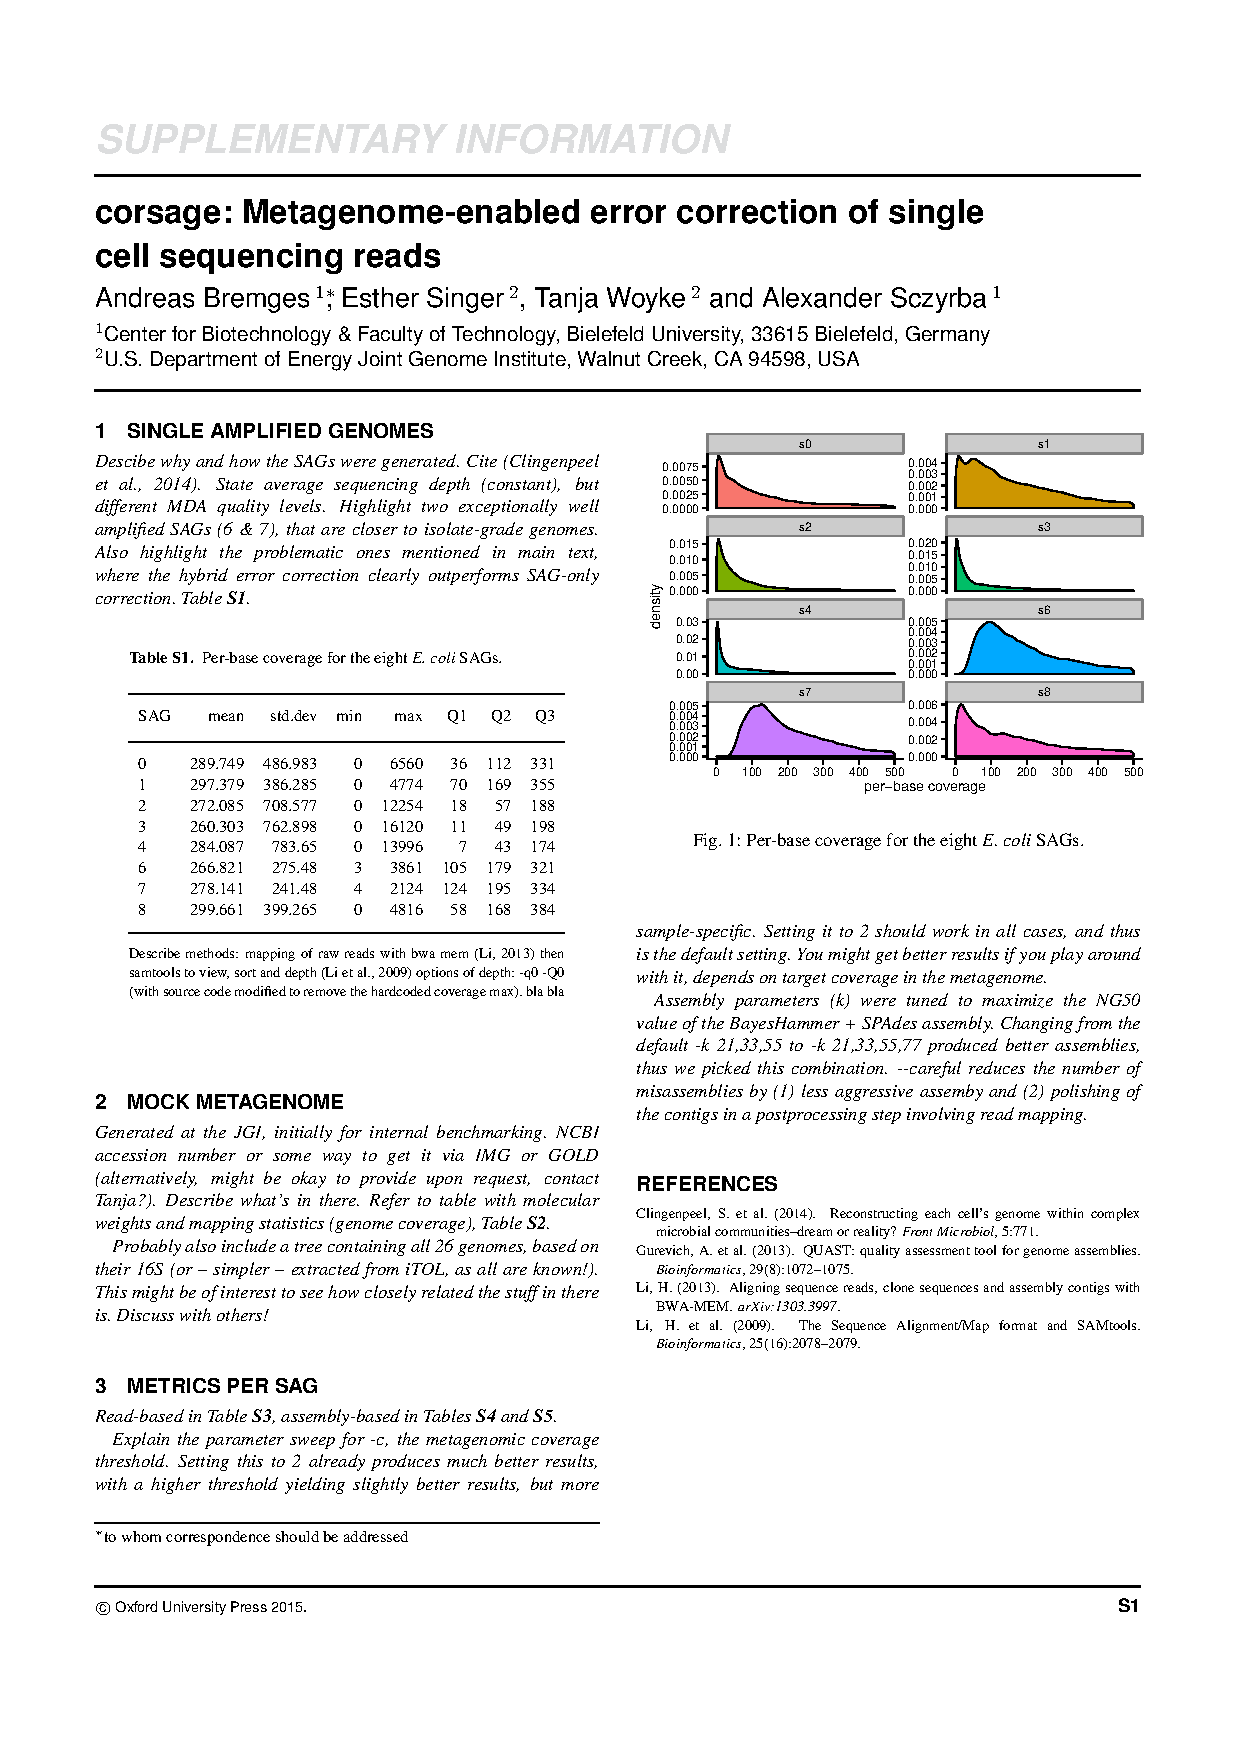
\includepdf[noautoscale,pages={1-}]{corsage_supp.pdf}
\end{document}
